\documentclass[a4paper,12pt]{article} 

%%% Работа с русским языком
\usepackage{cmap}                           % поиск в PDF
\usepackage{mathtext} 			 	       % русские буквы в формулах
\usepackage[T2A]{fontenc}               % кодировка
\usepackage[utf8]{inputenc}              % кодировка исходного текста
\usepackage[english,russian]{babel}  % локализация и переносы

%Матеша
\usepackage{amsmath,amsfonts,amssymb,amsthm,mathtools} % AMS
\usepackage{icomma} % "Умная" запятая

%\mathtoolsset{showonlyrefs=true} % Показывать номера только у тех формул, на которые есть \eqref{} в тексте.

%% Шрифты
\usepackage{euscript}	 % Шрифт Евклид
\usepackage{mathrsfs} % Красивый матшрифт

%% Свои команды
\DeclareMathOperator{\sgn}{\mathop{sgn}}

%% Перенос знаков в формулах (по Львовскому)
\newcommand*{\hm}[1]{#1\nobreak\discretionary{}
{\hbox{$\mathsurround=0pt #1$}}{}}

%%% Заголовок
\author{Муляревтч Андрей}
\title{Лабораторная работа 2.1.2

Определение $C_p / C_v$ методом адиабатического расширения}
\date{\today}

\begin{document}
	
\maketitle 
	
	
\newpage


\subparagraph*{Цель работы:}определение отношения $C_p / C_v$ углекислого газа  по измерения давления в стеклянном сосуде. Измерения производятся сначала после адиабатического расширения газа а затем после нагревания сосуда и газа до комнатной температуры. 
\subparagraph*{В работе используются:}стеклянный сосуд: U-образный жидкостный манометр; резиновая груша; газгольдер с углекислым газом. 

\begin{figure}[b!]	\label{plan2}
	
	\center{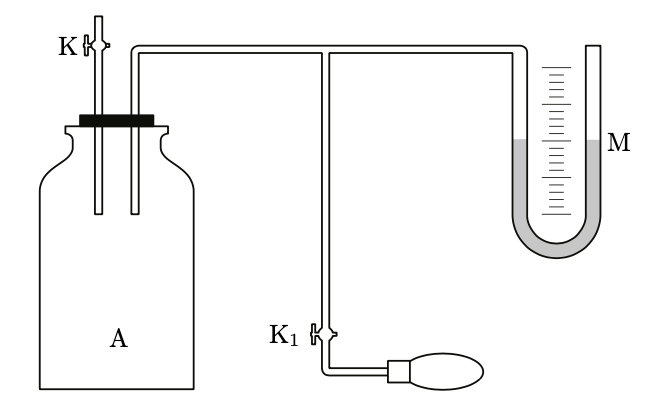
\includegraphics[width=1 \linewidth]{1.jpg}}
	\caption{Установка для определения $C_p / C_v$ методом адиабатического расширения газа}
	
\end{figure}



\subparagraph*{Экспериментальная установка.} Используемая для опытов экспериментальня установка состоит из стеклянного сосуда А (объёмом около 20 л), снабженного краном К, и U-образного жидкостного манометра, измеряющего избыточное давление газа в сосуде. Схема установки показана на Рис. 1. 

Избыточное давление создаётся с помощью резиновой груши, сосединённой с сосудом трубкой с краном $К_1$.

В начале опыта  в стеклянном сосуде А находится исследуемый газ при комнатной температуре $T_1$ и давлении $P_1$, несколько превышающем атмосферное давление  $P_0$. После открытия крана К, соединяющего сосуд А с атмосферой, давление и температура газа будут понижаться. Это уменьшение температуры приближённо можно считать адиабатическим. 

Для адиабатического процесса можно записать следующее уравнение: 

\begin{equation}\label{mk}
\left(\dfrac{P_1}{P_2}\right)^{\gamma - 1} = \left(\dfrac{T_1}{T_2}\right)^\gamma , 
\end{equation} 

где индексом "1" обозначено состояние после повышения давления в сосуде и выравнивания температуры с комнатной, а интексом "2"  $-$ сразу после открытия крана и выравнивания давления с атмосферным. 

После того, как кран К вновь отсоединит сосуд от атмосферы , происходит медленное изохорическое нагревание газа со скоростью, определяемой теплопроводностью стеклянных стенок сосуда. Вместе с ростом температуры растёт и давление газа. З время порядка $\Delta t_T$  (время установления температуры) система достигает равновесия, и установившаяся температура газа $T_3$ становится равной комнатной температуре $T_1$. 

Тогда используя закон Гей-Люссака для изохорического процесса и уравнение \eqref{mk} найдём $\gamma$:

\begin{equation}\label{acc}
\gamma = \dfrac{\ln(P_1 / P_0)}{\ln (P_1 / P_3)}.
\end{equation}

С учётом того, что $P_i = P_0 + \rho g h_i$ и пренебрегая членами второго порядка малости получим из \eqref{acc}:

\begin{equation}\label{r}
\gamma \approx \dfrac{h_1}{h_1 - h_2}.
\end{equation}


\newpage

\section*{Ход работы}

\subparagraph*{1.} Перед началом работы убедимся в том, что краны и места сочленений трубок достаточно герметичны. Для этого нужно наполнить баллон углекислым газом до давления, превышающего атмосферное  и перекроем кран $К_1$. По  U-образному манометру снимем зависимость давления $h$ в баллоне от времени $t$. По наблюдению было выявлено что за первые первые 60 секунд $\delta h$ $\approx$ 2 мм вод. ст. , за следущие 3 мин не изменилось, так что можно считать $\Delta t_T$ $\approx$ 60 сек.






\subparagraph*{2.} Откроем кран К на короткое время и закроем его снова. Подождём, пока уровень жидкости в манометре перестанет изменяться. Это произойдёт, когда температура газа в сосуде сравняется с комнатной, примерно через время $\Delta t_T$. Запишем разность уровней жидкости в манометре $h_2$. Проведём серию из 5--8 измерений сначала для времени открытия крана $\Delta t = 0,5 с$, а затем для $\Delta t = 1,0 с $. Далее так проведем по 1 опыту для больших значений $\Delta t$, которые зафиксируем с помощью телефонного секундомера. Так как отмерить время порядка 1с с большой точностью сложно из-за человеческой реакции, то мы проводим серию опытов для небольших $\Delta t$, после чего, пользуясь распределением Гаусса, выбираем наиболее вероятное значие для измеренных велечин, тем самым снижаем случайную ошибку примерно в $n$ раз, где $n$ -- кол-во опытов.


\begin{table}[h!]

	\begin{center}
	\caption{Экспирементальные данные для $\Delta t$ = 0,5 c}
	\begin{tabular}{|c|c|c|c|c|c|c|c|}
	\hline 
	h1, мм вд. ст. & 10 & 10,4 & 10,4 & 9,6 & 10 	& 10 & 10,4 \\ 
	\hline 
	h2, мм вд. ст. & 1,4 & 2 & 1,7 & 1,7 & 1,3 & 	1,6 & 1,9 \\ 
	\hline
	$\gamma$& 1,16 & 1,23 & 1,2 & 1,21 & 1,15 & 1,19 & 1,22 \\
	\hline 
	\end{tabular}
	
	\end{center}

\end{table}

Наиболее вероятное значение $\gamma$ для $\Delta t$ = 0,5 c: 1,21 \\
Случайная относительная погрешность в пределах $1 \sigma$: $\varepsilon$ = 1,2$\%$

\begin{table}[h!]

	\begin{center}
	
	\caption{Экспирементальные данные для $\Delta t$ = 1 c}
	
	\begin{tabular}{|c|c|c|c|c|c|c|c|}
	\hline 
	h1, мм вд. ст. & 10,4 & 10 & 10,4 & 10 & 10 & 10,4 & 10 \\ 
	\hline 
	h2, мм вд. ст. & 1,3 & 1,3 & 1,4 & 1,4 & 1,3 & 1,5 & 1,3 \\ 
	\hline 
	$\gamma$ & 1,14 & 1,15 & 1,16 & 1,16 & 1,15 & 1,17 & 1,15\\
	\hline
	\end{tabular}
	
	\end{center}

\end{table}

Наиболее вероятное значение $\gamma$ для $\Delta t$ = 1 c: 1,16 \\
Случайная относительная погрешность в пределах $1 \sigma$: $\varepsilon$ = 0,8$\%$


\begin{table}[h!]

	\begin{center}
	
	\caption{Экспирементальные данные для разынх $\Delta t$}
	
	\begin{tabular}{|c|c|c|c|}
	\hline 
	$h_1$ мм вд. ст.& $h_2$ мм вд. ст & $\gamma$ & $\Delta t$, с \\ 
	\hline 
	10,2 & 1,2 & 1,3 & 1,13 \\ 
	\hline 
	10,4 & 1,2 & 1,8 & 1,13 \\ 
	\hline 
	10,2 & 0,9 & 3,3 & 1,1 \\ 
	\hline 
	10,2 & 1 & 2,2 & 1,1 \\ 
	\hline 
	10,2 & 1 & 2,1 & 1,1 \\ 
	\hline 
	10 & 1,1 & 1,7 & 1,12 \\ 
	\hline 
	10 & 0,9 & 4,2 & 1,12 \\ 
	\hline 
	10,2 & 1,1 & 1,6 & 1,12 \\ 
	\hline 
	\end{tabular} 
	\end{center}

\end{table}


\newpage
По полученным данным вычислим используя формулу \eqref{r} вычислим $\gamma$ и построим график зависимости $\gamma(\Delta t)$ (График 1).


\begin{figure}[h!]

	\center{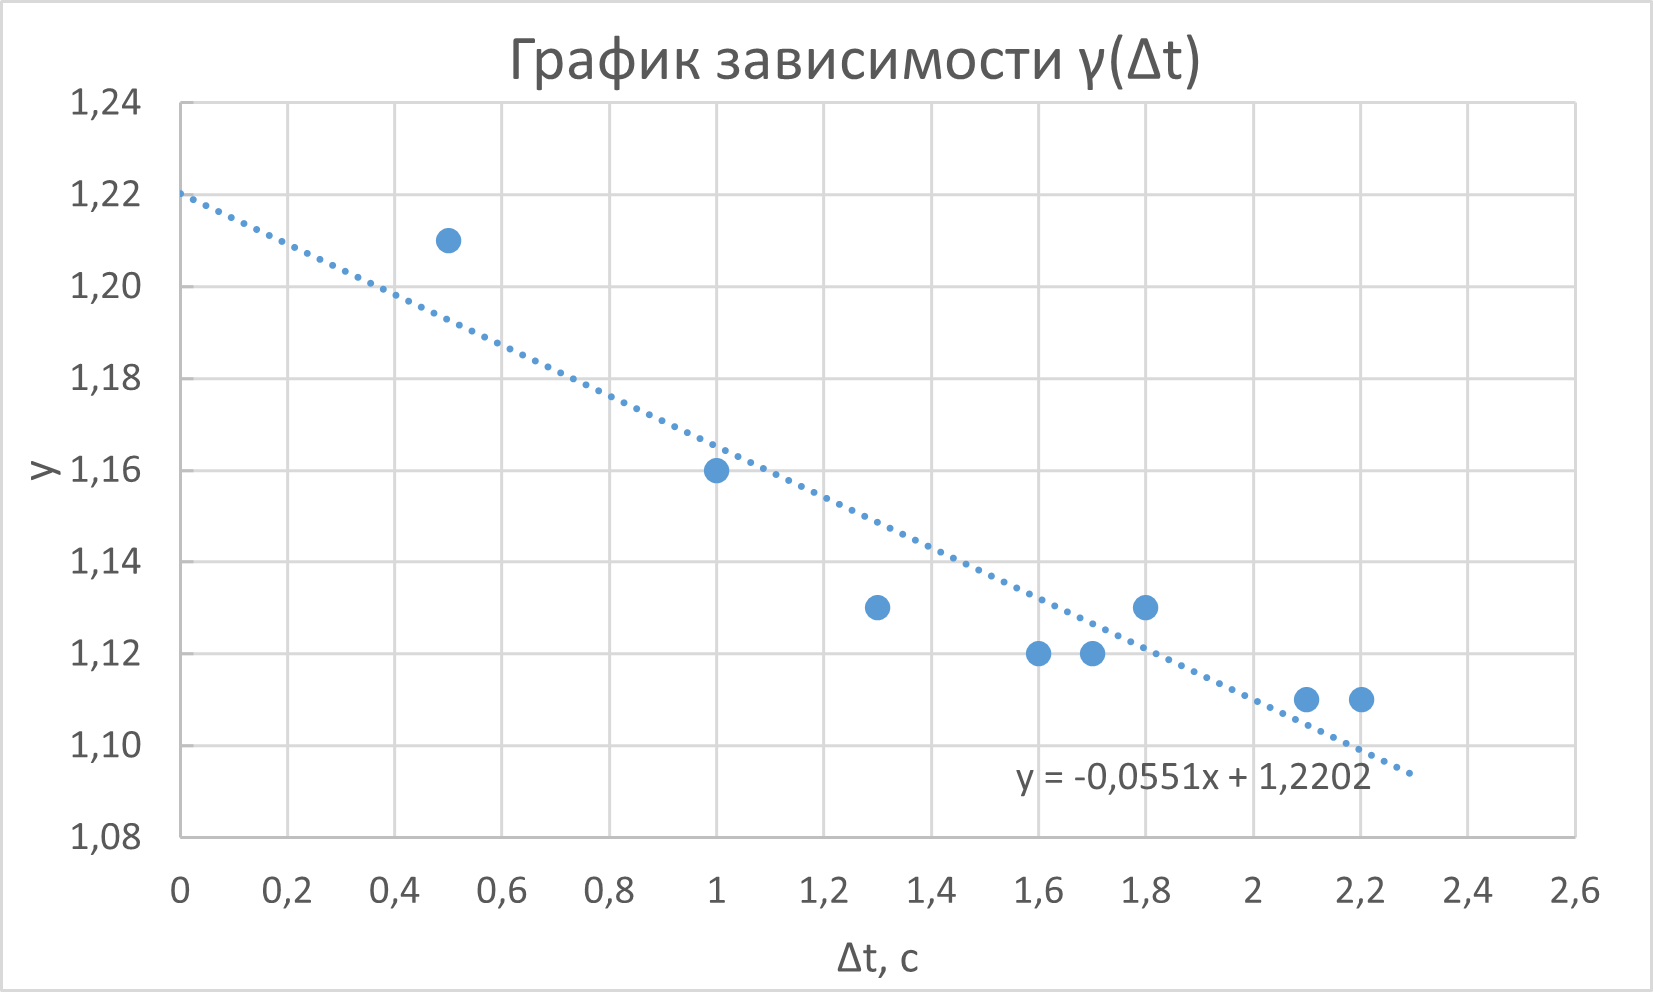
\includegraphics[width=\linewidth]{гамма_дельтат.png}}
	

\end{figure}



Теперь оценим вклад приборной погрешности при вычислении величины $\gamma$. Измерения $h_1$  и $h_2$ проводились с точностью 1мм. Пользуясь формулой \eqref{r} можно получить, что относительная погрешность искомой величины $$\dfrac{\sigma_\gamma}{\gamma} = \sqrt{\left(\dfrac{\partial\gamma(h_1, h_1 - h_2)}{\partial h_1}\sigma_{h_1}\right)^2 + {\left(\dfrac{\partial\gamma(h_1, h_1 - h_2)}{\partial h_1 - h_2}\sigma_{h_1 - h_2}\right)^2} }\approx 0.03$$

что даёт нам право пренебречь статистической погрешностью $\gamma$. Случайная погрешность измерения $\gamma$ для $\Delta t$ 0,5 и 1 с намного меньше приборной и ошибки из-за фактора человеческой реакции, так что ей можно принебречь.


Точность измерения времени, в течение которого газ выпускался из сосуда, оценивается точностью моей реакции, опыт показал, что эта величина составляет около 0.1 или даже меньше (поскольку интервал в 0.5 с примерно с такой точностью совпадает с временем прокручивания крана на полоборота), поэтому можно считать, что время измерено с точностью $\approx 7\%$

Тогда итоговая погрешность измерения показателя адиабаты составляет около $\sqrt{0.03^2+0.07^2} = 8\%$

	

\subparagraph*{3.} Окончательный результат следует получить экстраполяцией зависимости $\gamma$ от $t$ примерно к значению $\Delta t = 0,1 - 0,2 с$, когда давление уже почти сравнялось с атмосферным, но теплопроводность ещё не так сильно повлияла на уменьшение $\gamma$. Из полученного графика можно сделать вывод, что $\gamma_{CO_2} = 1.21 \pm 0.10$. В то время как табличное значение $\gamma_{CO_2} = 1.30$, т. е. совпадает с полученным значением в пределах погрешности. 


\section*{Вывод}
	

	Не смотря на то что результат совпал с табличным в пределах погрешности, точки на графике плохо апроксимируются прямой, возможно это связано с тем что по сути сам адиабатчиеский процесс проходит не во всем объеме а непосредственно возле крана и далее между слоями газа с одинаковыми параметрами($T$ и $p$), откуда можно сделать вывод что температура газа и его давление в колбе грубо говоря не являются интенсивными велечинами, и, соответсвенно теоритическое описание данной модели не верно, однако тот факт что результат получен правдивый говорит о том что данная модель уместна. Так же нужно заметить, что измерять время с помощью секундомера довольно неточно, данный эксперимент требует сложных измерительных конструкций для точного измерения интервалов времени чтобы оценить точность данной модели и уменьшить погрешность измерения времени, которая в свою очередь равна 7\% по грубым оценкам, что достаточно много. Так же нужно заметить что с ростом $\Delta t$ корректность полученных данных падает (данные полученные при $\Delta t$ > 3 с в расчет не брались)
\end{document}